\documentclass[a4paper]{article}
\usepackage[top=1in, bottom=1.25in, left=1.25in, right=1.25in]{geometry}
\usepackage{amsmath}
\usepackage{multicol}
\usepackage{graphicx}
\usepackage{subfig}
\usepackage{amssymb}
%\RequirePackage{ltxcmds}[2010/12/07]
%opening
\title{Linear Filtering in Frequency-Domain}
\author{ }
\date{ }
\begin{document}

\maketitle
\section{Introduction}
Linear filtering can be easily implemented in time-domain resorting to the use of finite impulse response (FIR) digital filters and convolution property as,
\begin{equation}
    y(n)= \sum\limits_{k=0}^{R-1} x(n-k)h\left(k\right),
    \label{genFIR}
\end{equation}
where $x(n)$ is the input signal, $h(k)$ is the FIR filter coefficients, $R$ is the length of FIR filter coefficients and $y(n)$ represents the filtered output signal.
Analysing this equation we can note that, for a block signal of length $R$, the required number of operations for the direct implementation of equation~\eqref{genFIR} evolves with $R^2$, $\mathcal{O}(R^2)$. This limitation imposed the emergence of algorithm, where the linear convolution is calculated faster than the directly implementing of \eqref{genFIR}.
In this sense, it is used the computation of linear filtering in frequency domain resorting to the use of fast Fourier transform (FFT) and inverse fast Fourier transform (IFFT) algorithms as
However, for long input sequence, the direct implementation of frequency domain filtering in real-time is limited by the limited memory of the digital processors.
Hence, the filtering in frequency-domain is implemented by sectioning or block the input signal, such that the practical implementation  of FFT and IFFT is feasible. In order to implement the non-cyclic convolution with the finite-length of cyclic convolution that the FFT provides, overlap-save and overlap-add method are use, enabling that the complexity evolves in log scale $\mathcal{O}(N\log_2N)$. The general method is to split the input signal into manageable blocks, then apply the FFT to to perform the linear convolution and at the end recombine the output blocks such that it is avoided the wrap-around errors due to the circular convolution imposed by FFT.

\section{Overlap-Save Method}
The overlap-save method can be computed in the following steps:
\begin{enumerate}
    \item   Step 1:
    \begin{itemize}
        \item   Determine the length $R$ of impulse response, $h(n)$;
    \end{itemize}
    \item   Step 2:
    \begin{itemize}
        \item   Define the size of FFT and IFFT operation, $N$;
    \end{itemize}
    \item   Step 3:
    \begin{itemize}
        \item   Determine the length of block $L$ to section the input sequence $x(n)$, considering that $N=L+R-1$;
    \end{itemize}
    \item   Step 4:
    \begin{itemize}
        \item   Pad $L-1$ zeros to the impulse response $h(n)$ to obtain the length $N$;
    \end{itemize}
    \item   Step 5:
    \begin{itemize}
        \item   Make the segments of the input sequences of length $L$, $x_i(n)$, where index $i$ correspond to the $i^{th}$ block. Overlap $R-1$ samples of the previous block at the beginning of the segmented block to obtain a block of length $N$. In the first block, it is added $R-1$ null samples;
    \end{itemize}
    \item   Step 6:
    \begin{itemize}
        \item   Compute the circular convolution of segmented input sequence $x_i(n)$ and $h(n)$ described as,
        \begin{equation}
            y_i(n)= x_i(n) \circledast h(n).
            \label{genFIR}
        \end{equation}
        This is obtained in the following steps:
        \begin{itemize}
            \item   Compute the FFT of $x_i$ and $h$ both with length $N$;
            \item   Compute the multiplication of $X_i(f)$ and the transfer function $H(f)$;
            \item   Compute the IFFT of the multiplication result to obtain the time-domain block signal, $y_i$;
        \end{itemize}     
    \end{itemize}
    \item   Step 7:
    \begin{itemize}
        \item   Discarded $R-1$ initial samples from the $y_i$, and save only the error-free $N-R-1$ samples in the output record.
    \end{itemize}
\end{enumerate}
%Following these steps, the input sequence is divided into blocks of length $L$ samples to be continuously processed. In the first block of length $L$, it is added $R-1$ null samples at the beginning of the block to obtain a block of length $N$ for the computation of FFT. The successive blocks are overlapped by $R$ previous samples.
%Then, an $N$-point FFT is computed for each data block. Then, the multiplication of $N$-point FFT and the transfer function is performed, followed by IFFT operations to obtain the time-domain block signal. $R-1$ initial samples are then discarded, and only the error-free $N-R-1$ samples are saved in the output record.
In the Figure~\ref{overlapSave} it is illustrated an example of overlap-save method.

\subsection{Frequency Response of Filter}
%\begin{figure*}[h!]
%    \centering
%    \subfloat[]{{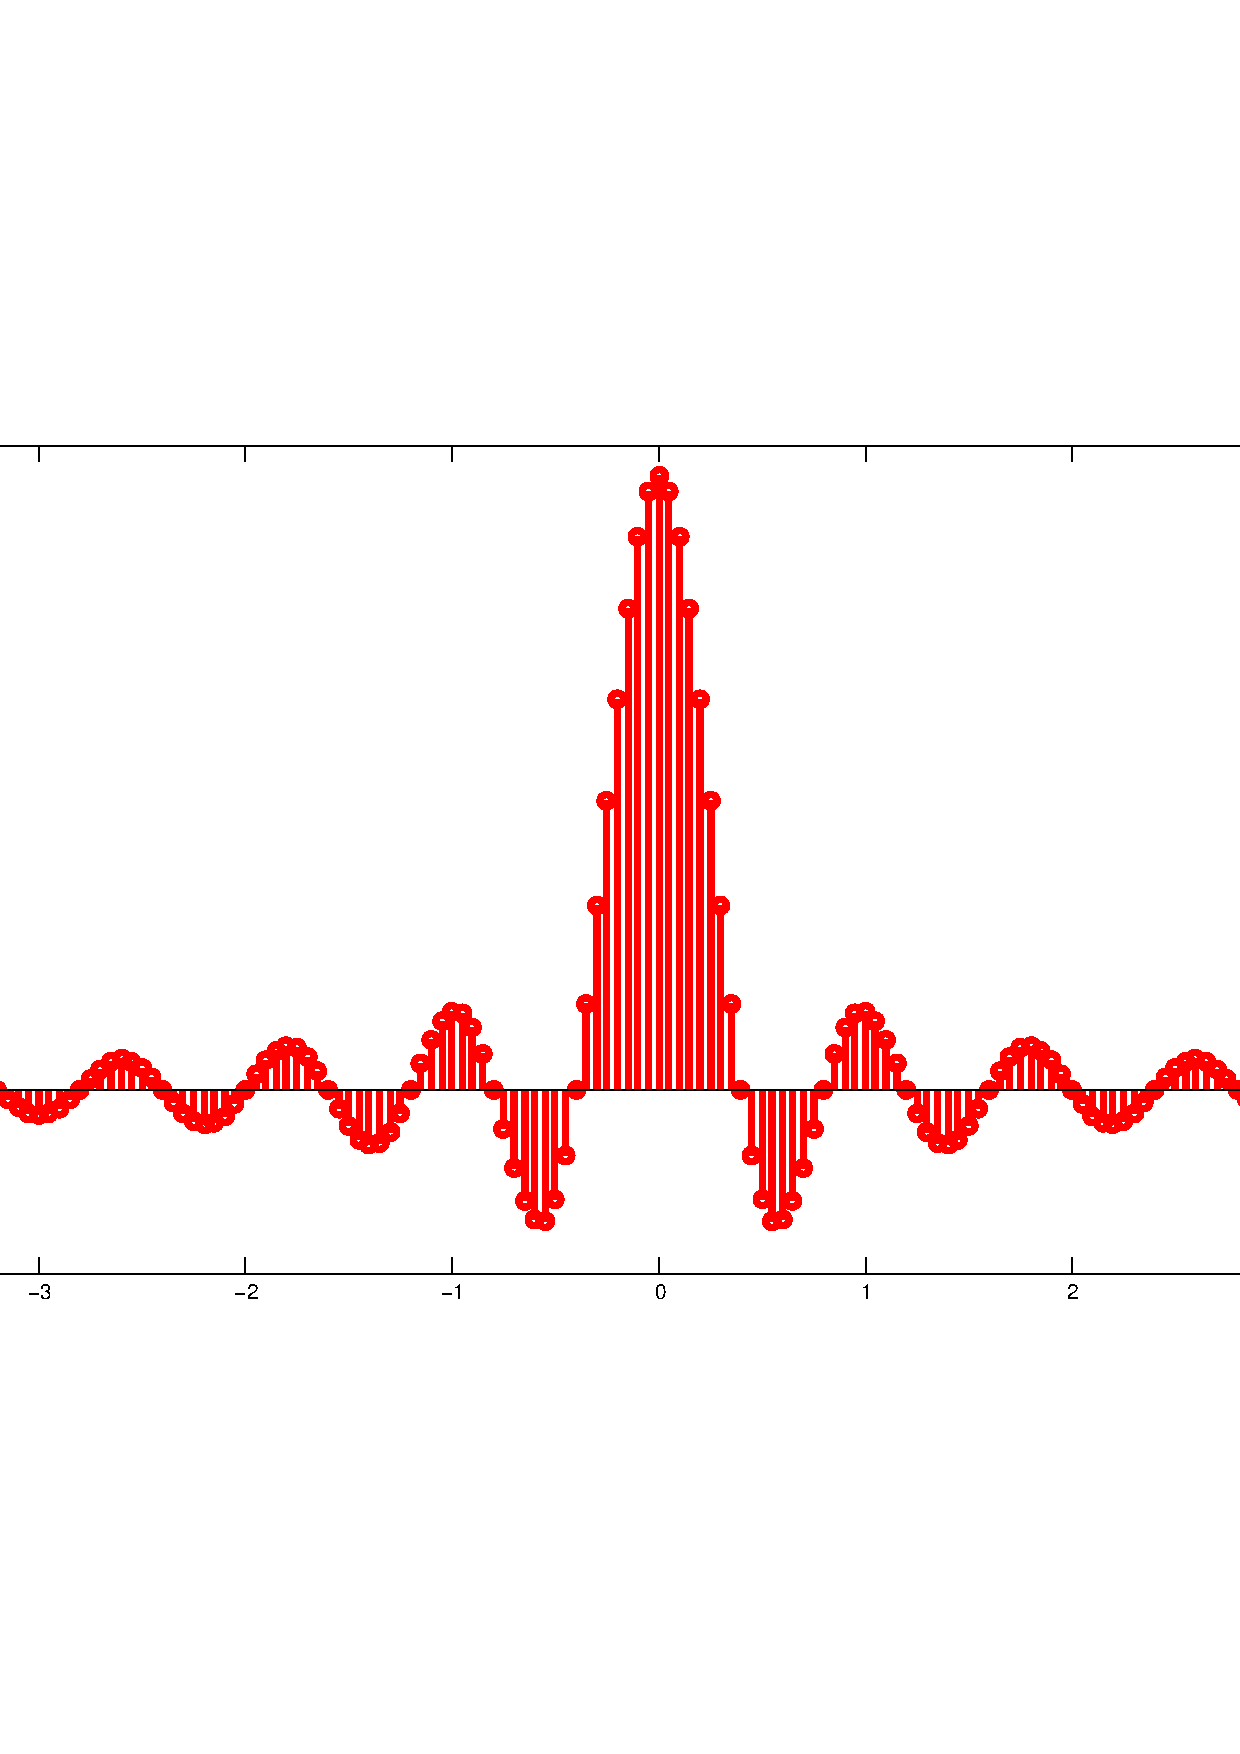
\includegraphics[width=.46\linewidth]{rc-td-filter-stem} }}%
%    \qquad
%    \subfloat[]{{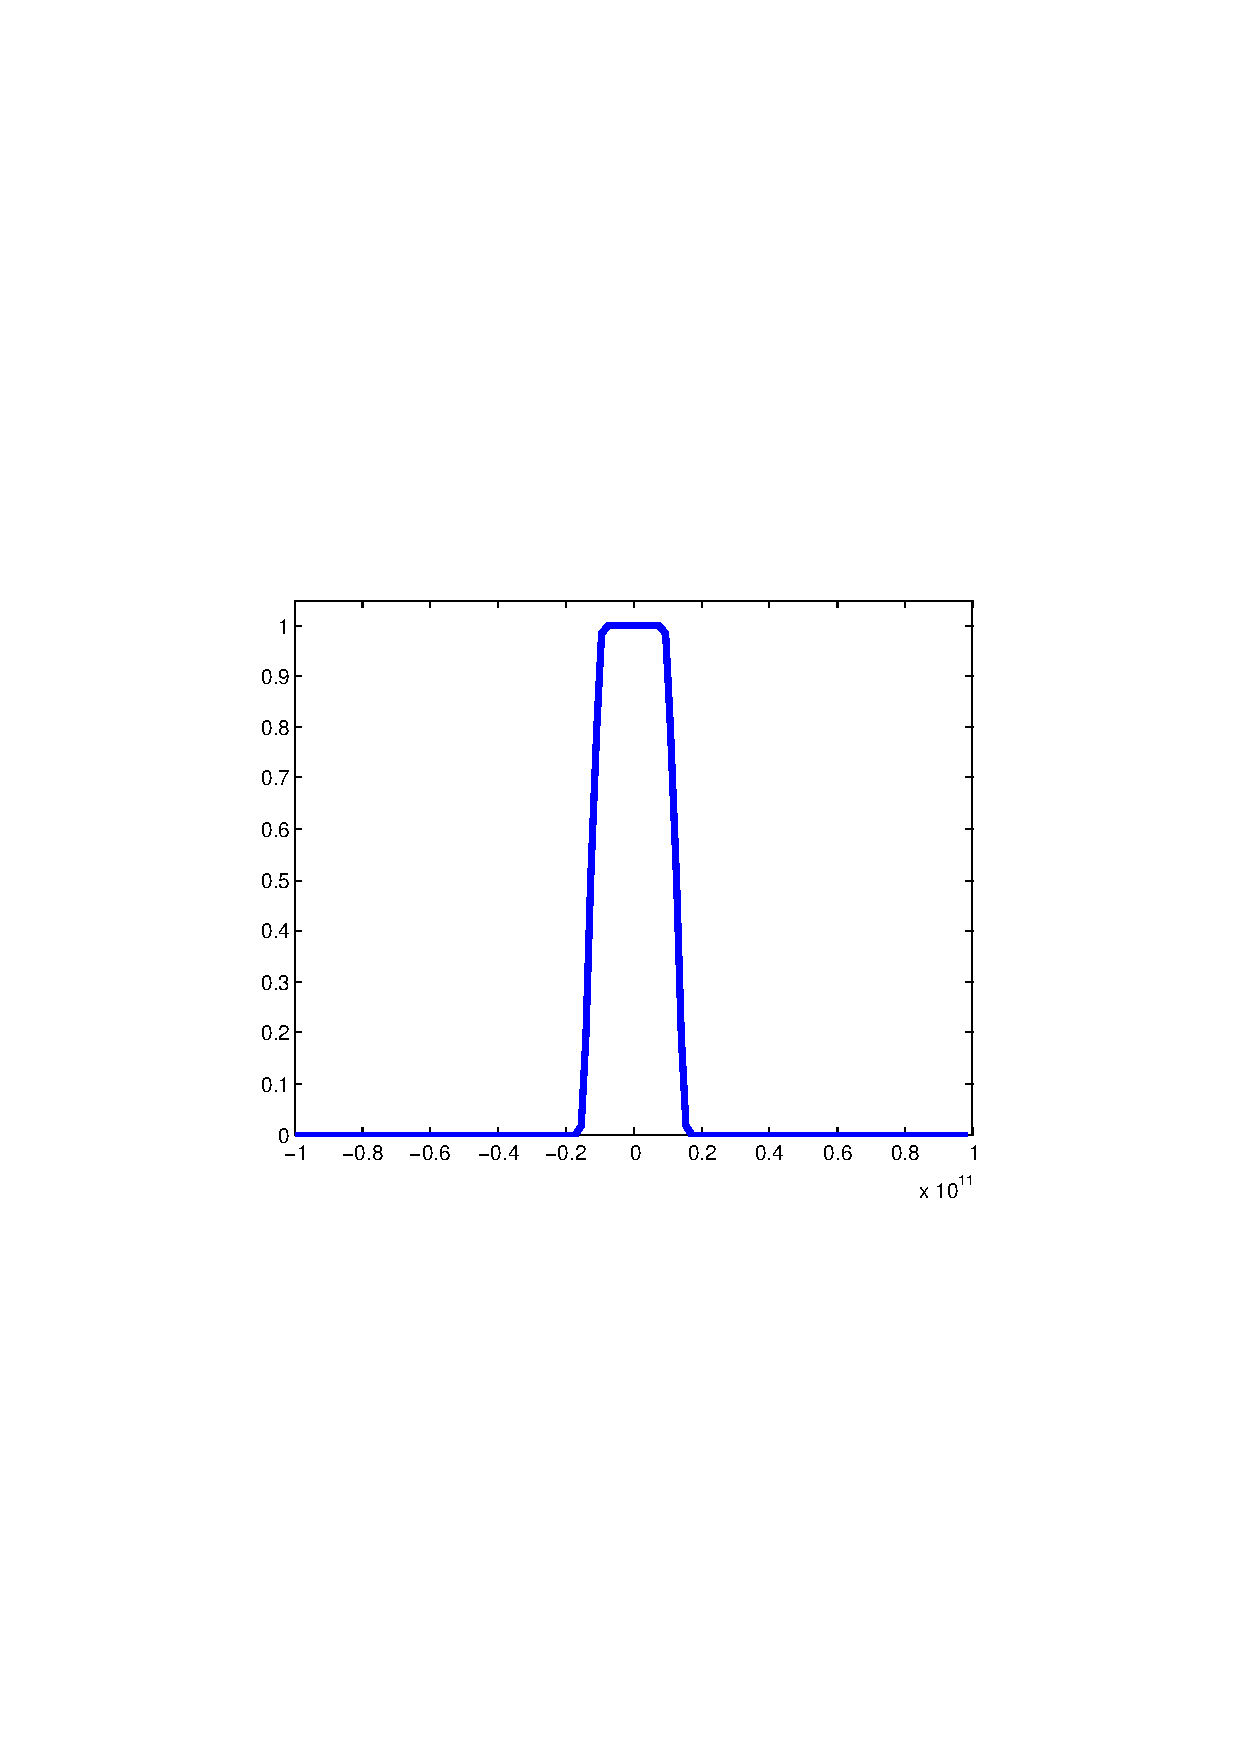
\includegraphics[width=.46\linewidth]{rc-fd-filter-SpS8} }}%
%    \caption{ a) Impulse response of raised cosine filter; b) Frequency response  of raised cosine filter. }%
%    \label{BER_InputPower}%
%\end{figure*}
\begin{figure}[t!]
    \centering
    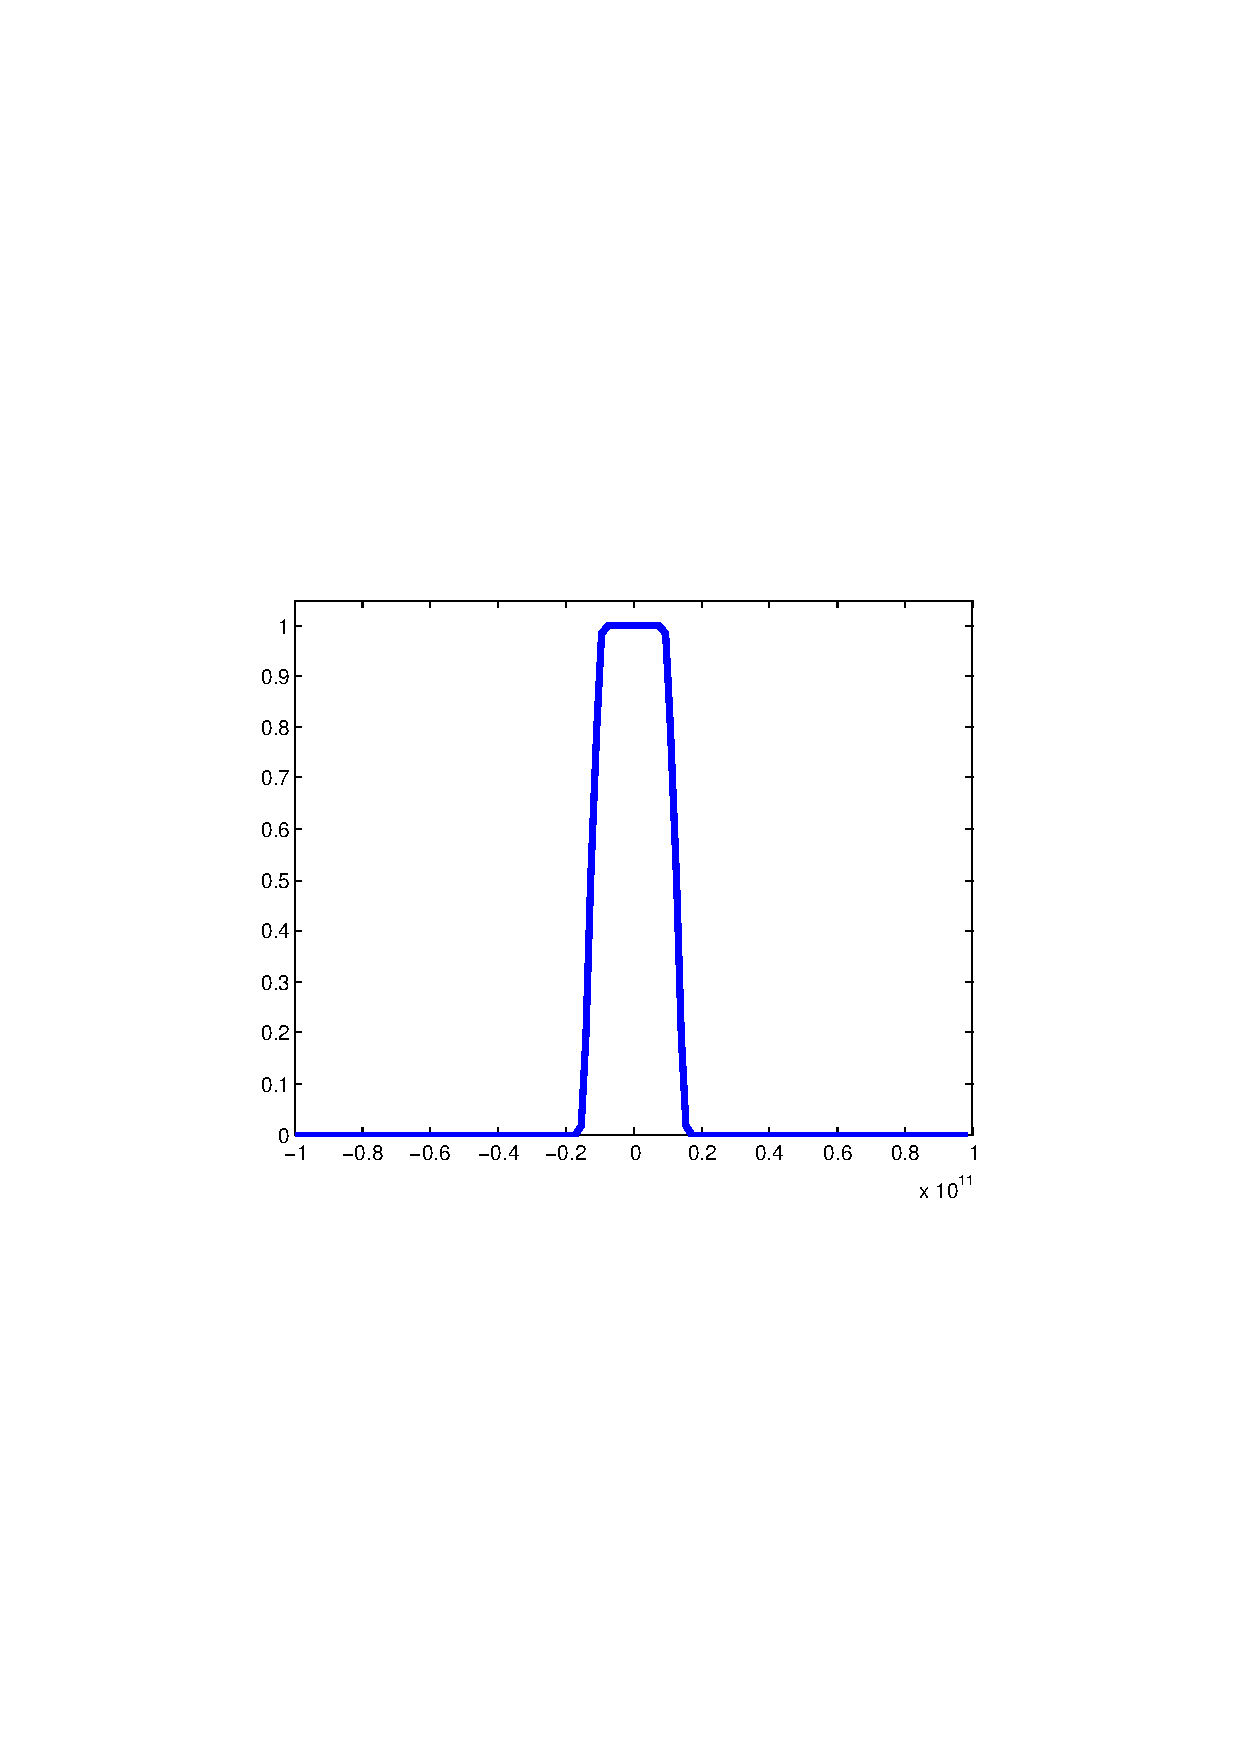
\includegraphics[width=6cm]{rc-fd-filter-SpS8}
    \caption{Frequency response of raised-cosine filter.}
    \label{freq_rc}
\end{figure}

The frequency response of filter can be directly defined by using the frequency-domain formula, or it can be equivalently calculated from the FFT of impulse response of the filter. In this sense, we present an example of FIR filter (\textit{raised-cosine filter}) to illustrate these two cases.

\subsubsection{Frequency-domain Formula}

The frequency-domain description of raised-cosine filter can be given as,
%\[ H(f) =
%  \begin{cases}
%    1,       & \quad \left|f\right| \leq \frac{1-\beta}{2T} \\
%    \frac{1}{2}\left[ 1+\cos\left(\frac{\pi T}{\beta}\left[\left|f\right| - \frac{1-\beta}{2T}\right]\right)\right],  & \quad \frac{1-\beta}{2T} < \left|f\right| \leq \frac{1+\beta}{2T}\\
%    0, & \quad \text{otherwise}
%  \end{cases}
%\]
$$
H(f) = \left\{
    \begin{array}{ll}
        1,       & \quad \left|f\right| \leq \frac{1-\beta}{2T} \\
    \frac{1}{2}\left[ 1+\cos\left(\frac{\pi T}{\beta}\left[\left|f\right| - \frac{1-\beta}{2T}\right]\right)\right],  & \quad \frac{1-\beta}{2T} < \left|f\right| \leq \frac{1+\beta}{2T}\\
    0, & \quad \text{otherwise}
    \end{array}
\right.
$$
where, $f$ is the frequency, $0 \leq \beta \leq 1$ corresponds to the roll-off factor and $T$ is the reciprocal of the symbol-rate.
A plot of direct implementation of frequency response of raised-cosine filter is presented in Figure~\ref{freq_rc}, for a roll-off factor of 0.3.
The frequency response, $H(f)$, calculated for $N$ frequency bins, which can be defined as,
\begin{equation}
    f= -\frac{fwindowTF}{2}:\frac{fwindowTF}{N}:\left(\frac{fwindowTF}{2}-\frac{fwindowTF}{N}\right),
    \label{freq}
\end{equation}
where $fwindowTF$ is the sampling frequency. This, imposes that the length of $H(f)$ is $N$ as expected for the $N$-point FFT and the transfer function multiplication.
\subsubsection{FFT of Impulse Response}
Alternatively to the frequency-domain formula, we can obtain the frequency response of filter by calculating the FFT of its impulse response. In the case of raised-cosine filter, the impulse response is given as,

\begin{equation}
    h(t)= \frac{\sin(\pi t/T)}{\pi t/T}\frac{\cos(\pi t \beta/T)}{1-(2\beta t/T)^2},
    \label{hn}
\end{equation}
where $t$ is the time. Figure~\ref{td_rc} shows a plot of impulse response of raised-cosine filter for a roll-off factor of 0.3.
\begin{figure}[h!]
    \centering
    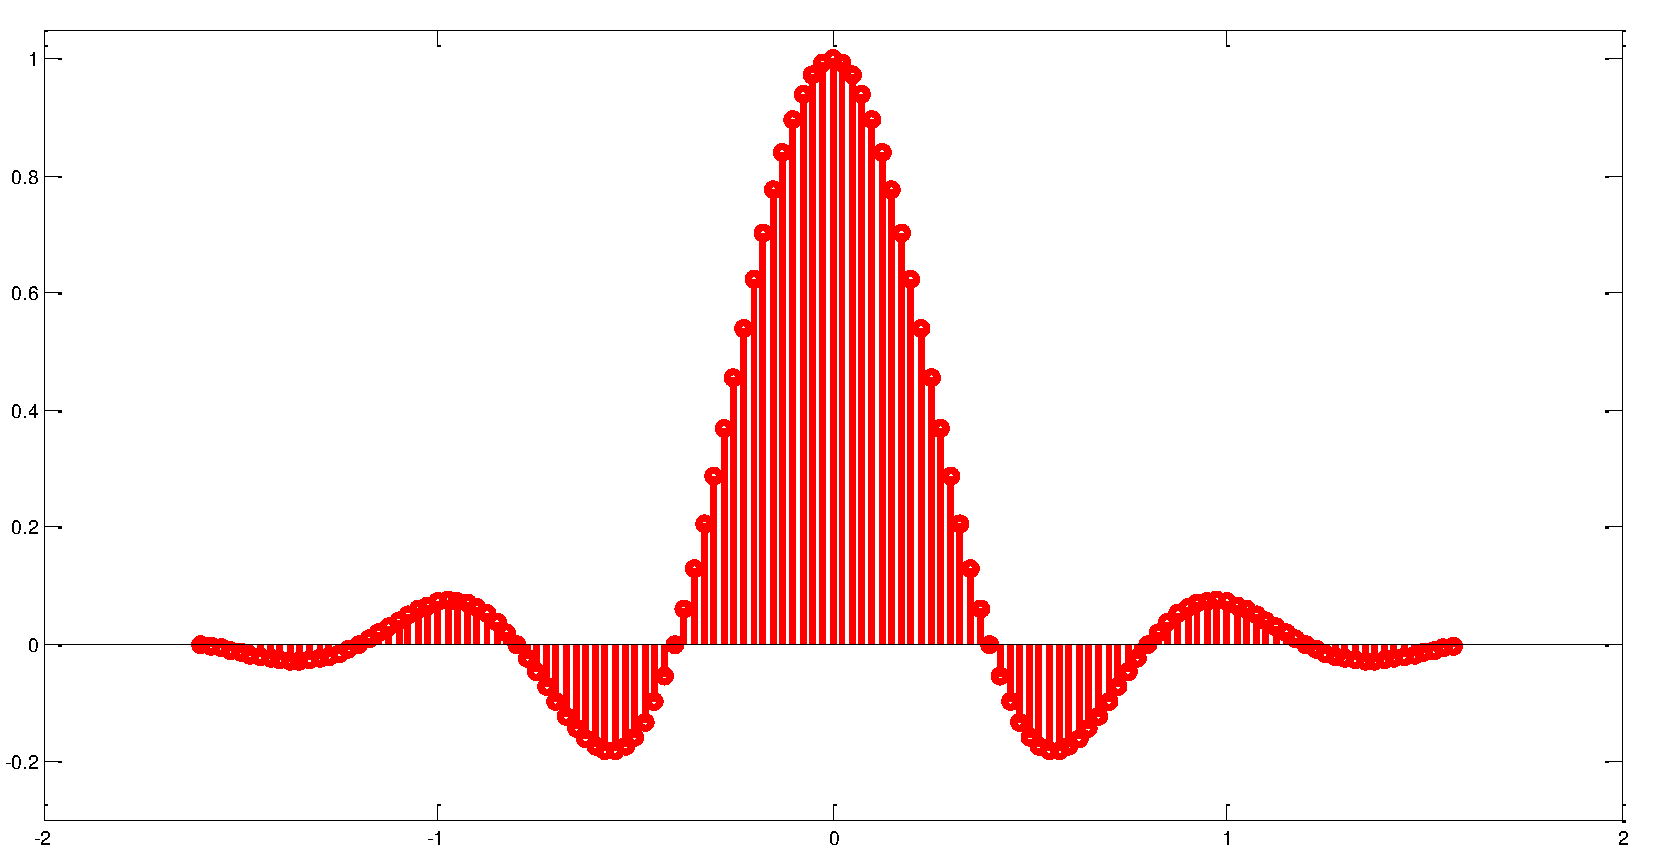
\includegraphics[width=8cm]{rc-td-filter-stemv2}
    \caption{Impulsee response of raised-cosine filter.}
    \label{td_rc}
\end{figure}
Before calculating the FFT of the impulse response we must zero-pad the impulse response, which has the length $R$, to the length $N$. In this case $N$ is the FFT length, which is efficiently defined as power of 2. The zero-padding process can be performed by appending $L-1$ zeros at the end of impulse response, as shown in the Figure~\ref{zp-hn}.

\begin{figure}[t!]
    \centering
    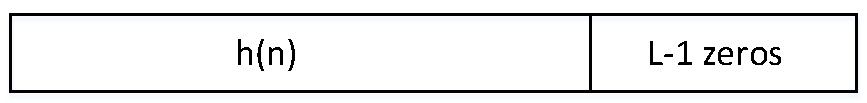
\includegraphics[width=6cm]{zp-hn}
    \caption{Zero-padding of impulse response $h(n)$.}
    \label{zp-hn}
\end{figure}

In both cases, the frequency response of the filter will be limited to the frequency interval $fwindowTF$, [$-\frac{fwindowTF}{2}$, $\frac{fwindowTF}{2}$], and this range show us the $N$ frequency components obtained from FFT. The minimum frequency bin is $-\frac{fwindowTF}{2}$ and the maximum bin is $\frac{fwindowTF}{2}$, in which $fwindowTF$ corresponds to the sampling frequency. We can note that the spectral width of $H(f)$ is $fwindowTF$, which is the inverse of sampling period, $\mathop{dt}$. It is also important to note that, for a given sampling frequency, the frequency resolution, $\Delta f$, of $H(f)$ depends on the parameter $N$ and it increases with $N$, $\Delta f=\frac{fwindowTF}{N}$.
\begin{figure}[h]
    \centering
    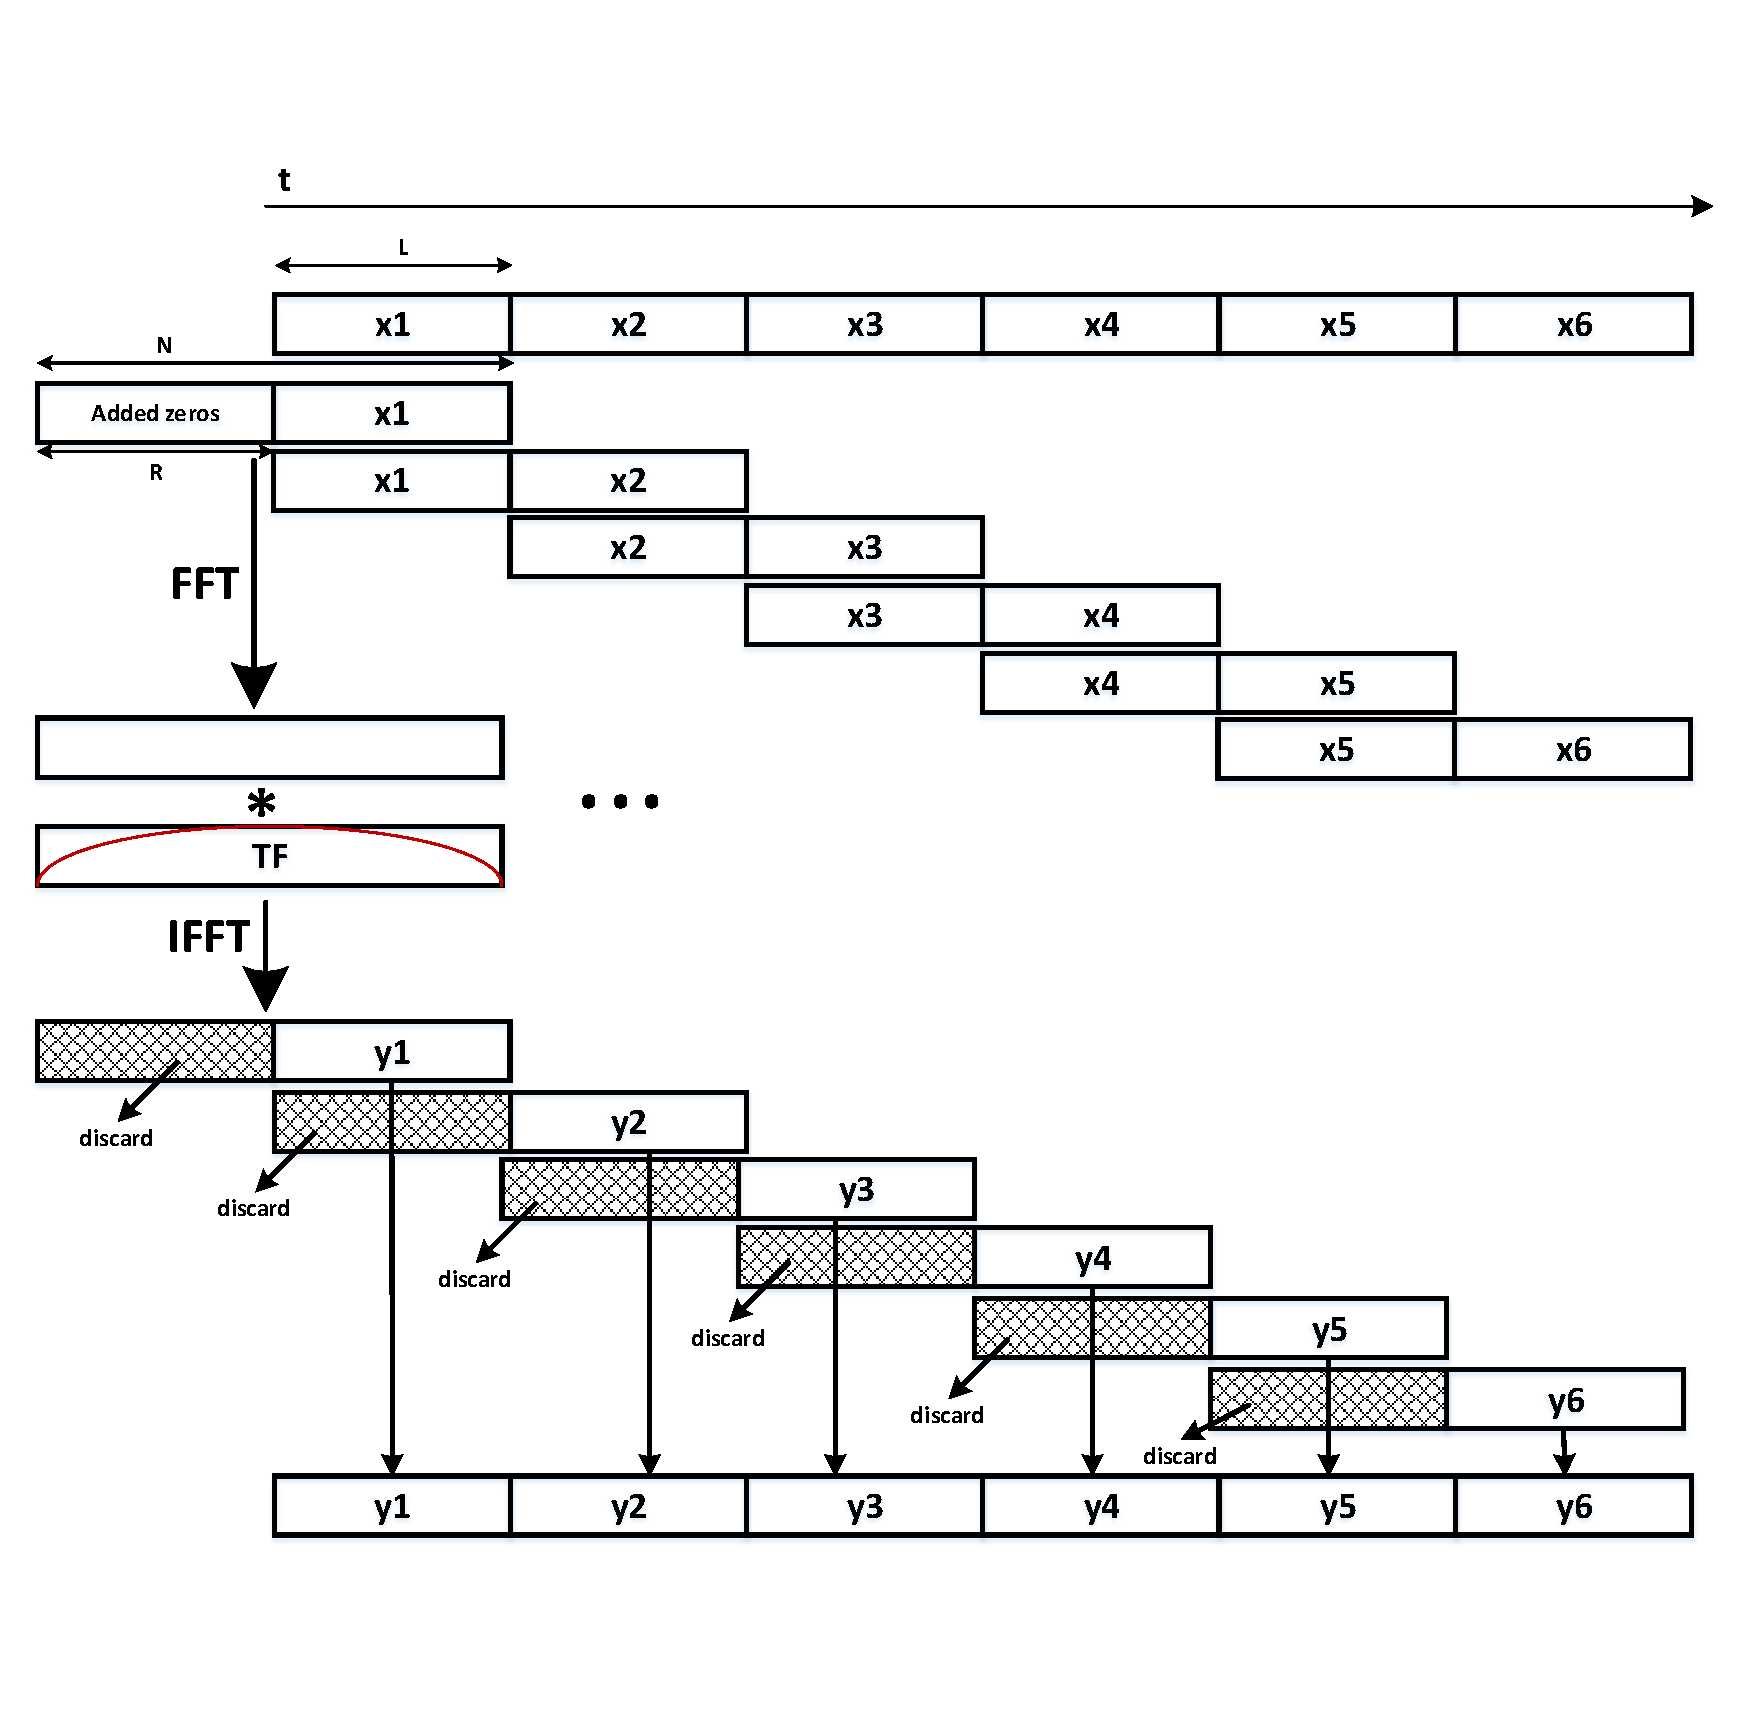
\includegraphics[width=15cm]{overlap-savev2}
    \caption{Illustration of Overlap-save method.}
    \label{overlapSave}
\end{figure}
 \begin{thebibliography}{1}
  \bibitem{notes} Blahut, R.E. {\em Fast Algorithms for Digital Signal Processing}, Addison-Wesley, Reading, MA,
1985.
  \bibitem{notes} Steven W. Smith. {\em The Scientist and Engineer's Guide to Digital Signal Processing.} California Technical Publishing, San Diego, CA, USA, 1997.

  \end{thebibliography}

\end{document}

